\chapter*{Introducere} 
\addcontentsline{toc}{chapter}{Introducere}

Modele bazate pe arhitecturi de tip ``\textit{Transformer}'' au revoluționat modul prin care textul este generat. Deoarece aceste modele sunt capabile să înțeleagă importanța fiecărui token dintr-o secvență prin algoritmul de ``\textit{Attention}'' (Vaswani et al.) \cite{vaswani2023attentionneed}, ele sunt capabile să genereze texte foarte credibile, precum și răspunsuri corecte și personalizate la întrebări. Acestea au fost aplicate cu succes major în domenii precum procesarea textului în modele precum seria ``\textit{GPT}'' (Radford et al.) \cite{radford2018improving}, dar și a imaginilor precum modelele ``\textit{DALL-E}'' (Radford et al) \cite{ramesh2021zeroshottexttoimagegeneration}.

Modelele generative pentru imagini din ultimii ani folosesc cu mult succes o metodologie bazată pe prezicerea pixelilor din zgomot, cel mai des dintr-o distribuție Gaussiană. Procedura de preprocesare a datelor implică crearea a $n$ instanțe ce conțin gradual din ce în ce mai mult zgomot în ele. În antrenare, modelele au sarcina de a inversa acest proces. Acest procedeu se numește ``\textit{Diffusion}'' (Ho et al.) \cite{ho2020denoisingdiffusionprobabilisticmodels}.

Revenind la muzică, pentru procesarea datelor pot fi folosite diverse tehnici. Deseori, este folosită analiza spectrală folosind transformări fourier de scurtă durată. Aceste transformări reușesc să extragă frecvențele prezente într-o undă oarecare, fapt ce ne ajută în a înțelege cum aceasta este compusă. În urma unei asemenea analize spectrale, vom obține o spectrogramă aferentă secvenței audio.

În această lucrare propun un model generativ pentru procesare audio, ce acceptă text drept instrucțiuni de generare. Acest model folosește conceptele definite anterior pentru a-și atinge scopul.

\section{Reprezentări ale datelor}

Sunetul reprezintă vibrația unui mediu de transmisie. Deseori, acest mediu este aerul, însă poate fi și altul. Vibrația mediului poate fi reprezentat ca o undă, compusă dintr-o sumă de alte unde de diverse intensități, ce urmăresc axa timpului. O undă sonoră poate fi reprezentată în mod digital prin capturarea sa de către un microfon. Transformarea acestui semnalul dintr-unul analog într-unul analog se numește ``conversie analog-digitală'', din care rezultă un șir de octeți. Acest șir de octeți poate fi utilizat și manipulat de către echipamente electrice și electro-logice.

Invers, pentru redarea acestei secvențe de octeți, putem realiza o conversie inversă - o ``conversie digital-analogică'' - pentru a reda sunetul precum cel original (excluzând atenuările și zgomotul obținut la capturare). Capturarea unei unde în mod exact în schimb este un proces foarte intens pe spațiul de stocare, așa că pentru prelucrare și producție sunt folosite diverse reprezentări.

Muzica în sine este compusă și ea la rândul său din sunete. În producerea și prelucrarea ei, pe lângă reprezentarea în formă de undă, mai putem folosi forma spectrală, obținută prin folosirea transformărilor Fourier pe intervale scurte de timp.

\begin{figure}[H]
    \centering
    \begin{subfigure}{.5\textwidth}
        \centering
        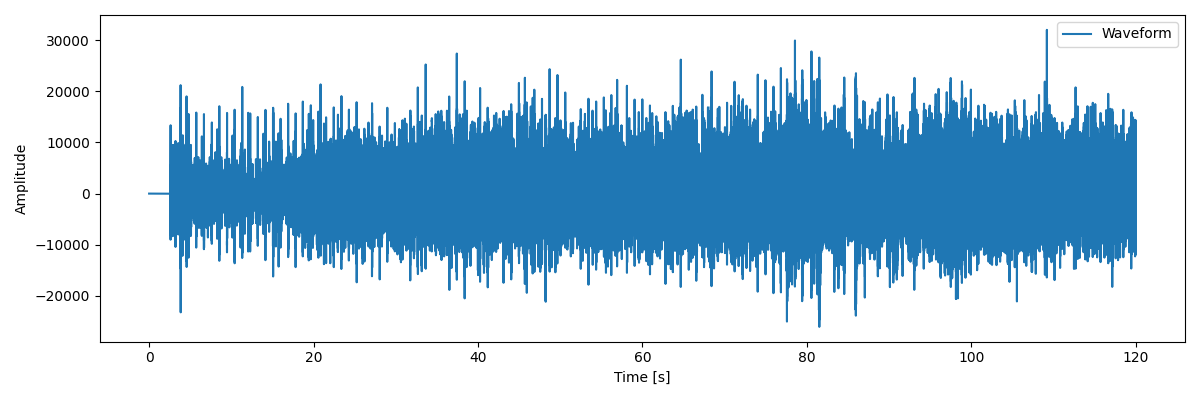
\includegraphics[width=1\linewidth]{waveform.png}
        \caption{Suma a două unde sonore}
        \label{waveform}
    \end{subfigure}%
    \begin{subfigure}{.5\textwidth}
        \centering
        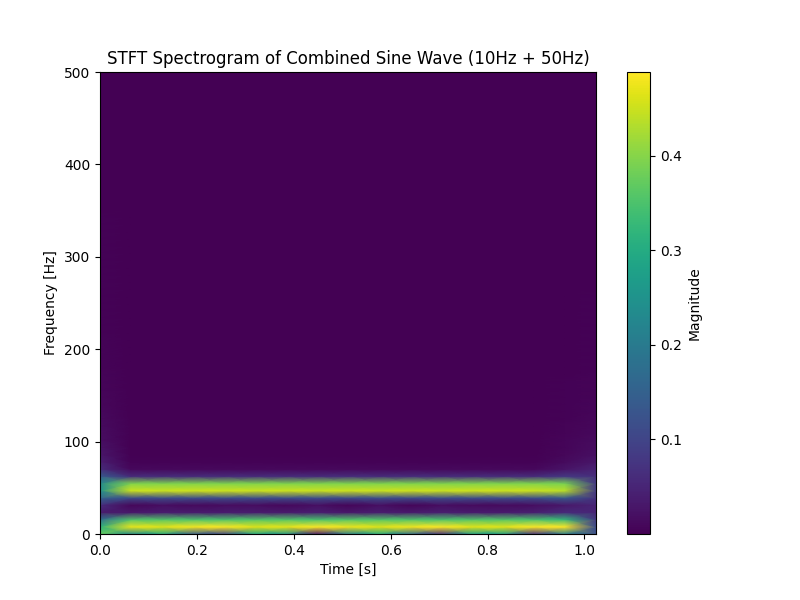
\includegraphics[width=1\linewidth]{spectrogram.png}
        \caption{Spectrograma figurii \ref{waveform}}
        \label{spectrogram}
    \end{subfigure}
    \caption{Reprezentări fidele realității}
    \label{reprezentări-fidele-realității}
\end{figure}

Aceste reprezentări pot reproduce cu fidelitate înaltă sunetul original, precum și emoția, improvizările și imperfecțiunile artistului. Pentru o reproducere fidelă teoriei, se folosesc în schimb partituri, gramatici, piano-rolls și MIDIuri. Aceste formaturi renunță la imperfecțiuni, ceea ce le face uneori mai puțin dezirabile pentru anumite genuri muzicale.

\begin{figure}[H]
    \centering
    \begin{subfigure}{.5\textwidth}
        \centering
        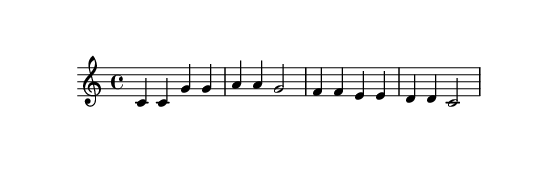
\includegraphics[width=1\linewidth]{partiture.png}
        \caption{Partitură}
        \label{partiture}
    \end{subfigure}%
    \begin{subfigure}{.5\textwidth}
        \centering
        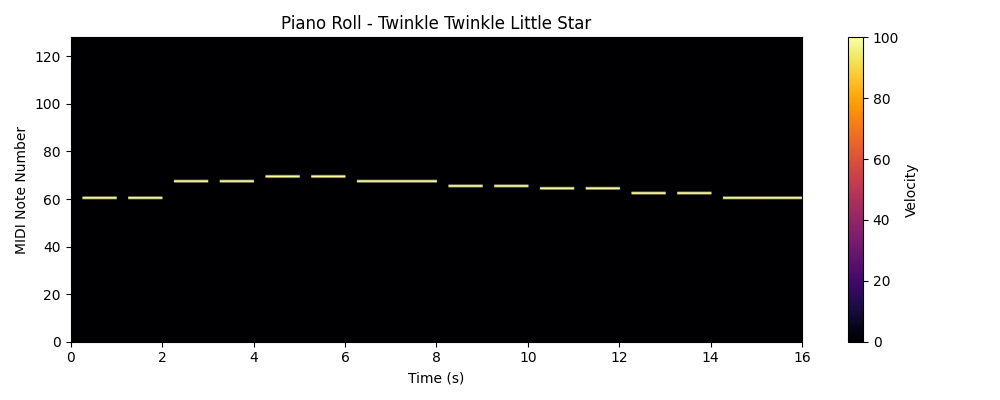
\includegraphics[width=1\linewidth]{pianoroll.png}
        \caption{Piano roll}
        \label{pianoroll}
    \end{subfigure}
    \caption{Reprezentări fidele teoriei}
    \label{reprezentări-fidele-teoriei}
\end{figure}

Deorece muzica este o știință ce se bazează pe modele matematice, dar în același timp este și o artă, trebuie găsit un balans între reprezentările perfecte și imperfecte. Acest balans este necesar pentru asigura reproducerea unei compoziții muzicale.
